% !TeX spellcheck = sk_SK
% LaTeX document class
\documentclass[nominted]{uniza}

%-------------------------------------------------------
%             Abbreviation and term database
%-------------------------------------------------------
% !TeX spellcheck = sk_SK

%----------------------------------------------------------
%						Slovník
%----------------------------------------------------------

\DeclareAcronym{viskozita} {
	short = Viskozita,
	long = {Fyzikálna veličina, miera odporu tekutiny deformovať sa pod vplyvom šmykových (tangenciálnych) napätí. Prejavuje sa vnútorným trením.},
	class = dict
}

\DeclareAcronym{zhlukovanie} {
	short = Zhlukovanie,
	long = {Trieda metód strojového učenia, ktoré v daných dátach hľadajú zhluky.},
	extra = {\begin{subdict}
			\item[Hierarchické zhlukovanie] Metódy zhlukovania, kde rozdelenie do zhlukov má hierarchickú štruktúru.
			\item[Fuzzy c-means zhlukovanie] Verzia algoritmu k-means pre fuzzy zhlukovanie.
		\end{subdict}
	},
	class = dict
}

\DeclareAcronym{triedenie} {
	short = Triedenie,
	long = {Pojmy v slovníku sa automaticky triedia podľa abecedy. \hl{Ale pozor: triedenie sa deje prvého argumentu makra \texttt{DeclareAcronym} -- nie podľa poľa \texttt{short}.}},
	class = dict
}

\DeclareAcronym{slovník_pojmov} {
	short = Slovník pojmov,
	long = {
	\hl{Slovník pojmov je nepovinný. Na jeho odstránenie stačí zmazať všetky zadefinované pojmy v súbore modules/abbterms.tex.}},
	class = dict
}

%----------------------------------------------------------
%						Skratky
%----------------------------------------------------------

\DeclareAcronym{MAE} {
	short = MAE,
	long = stredná absolútna chyba (\angl{mean absolute error}),
	class = abbrev
}

\DeclareAcronym{ANN} {
	short = ANN,
	long = umelá neurónová sieť (\angl{artificial neural network}),
	class = abbrev
}

\DeclareAcronym{MLP} {
	short = MLP,
	long = {viacvrstvový perceptrón, viacvrstvová neurónová sieť (\angl{multi-layer perceptron})},
	class = abbrev
}


%-------------------------------------------------------
%            Súbory s bibliografickými informáciami
%-------------------------------------------------------
\addbibresource{bibliography.bib}

%-------------------------------------------------------
%                  Jazykové nastavenia
%-------------------------------------------------------
\usepackage[english,slovak]{babel}

%-------------------------------------------------------
%                Potrebné balíčky
%-------------------------------------------------------

\usepackage{etoc}

%-------------------------------------------------------
%                Informácie o dokumente
%-------------------------------------------------------


\title{Názov práce}
\subtitle{Podnázov práce (ak existuje)}
\author{Jozef Mrkva}
\keywords{Vložte minimálne 4 kľúčové slová výstižne charakterizujúce spracovanú tému.}
\keywordsSecLang{Insert the minimum of 4 keywords that accurately characterize your topic.}

\keywordsName{Kľúčové slová}
\keywordsNameSecLang{Keywords}

\faculty{Elektrotechnická fakulta}
\department{Katedra riadiacich a informačných systémov}

% školiace pracovisko, ak je iné než katedra:
%\supervisorinst{
%	SIEMENS\\
%	Kompetenčné centrum Žilina
%}

\facultyshort{EF}
\location{Žilina}

\doctype{Diplomová práca}
\docid{Evidenčné číslo práce}
\supervisor{Titul, vedúci práce}
%Meno konzultanta (ak existuje):
\consultant{Titul, konzultant práce}

\academicyear{2018/2019} % akademický rok
\submissionyear{2019} % rok odovzdania práce
% Študijný program:
\studyprogramme{Riadenie procesov}
% Študijný odbor:
\fieldofstudy{5.2.14 Automatizácia}

% Abstrakt v hlavnom jazyku
\abstract{Abstrakt}{
Abstrakt obsahuje informáciu o cieľoch práce, jej stručnom obsahu a v závere abstraktu sa charakterizuje splnenie cieľa, výsledky a význam celej práce. Abstrakt sa píše súvisle ako jeden odsek a jeho rozsah je spravidla 100 až 500 slov.
}

% Abstrakt v cudzom jazyku (anglickom, nemeckom, ...)
\abstractSecLang{Abstract}{
In this place insert the text of the abstract in English or another foreign language. Sem vložte text abstraktu v angličtine, prípadne v inom cudzom jazyku.
}

%Dátum odovzdania práce
\date{Dátum odovzdania práce}

\acknowledgements{
	Poďakovanie nie je povinné. Ak nemá byť zahrnuté, stačí túto časť zakomentovať.
}

%-------------------------------------------------------
%		 Vybrané metadáta zapíšeme aj do dokumentu.
%-------------------------------------------------------

\hypersetup{
	pdfauthor={\Author},%
    pdftitle={\Title},%
    pdfsubject={\Doctype},%
    pdfkeywords={\Keywords},%
    pdfproducer={LaTeX},%
%    pdfcreator={pdfLaTeX}
}

%-------------------------------------------------------
%						Includeonly
%-------------------------------------------------------

%\includeonly{
%kap_uvod
%}

%-------------------------------------------------------
%		Korektné zalamovanie spojok na konci riadku.
%-------------------------------------------------------
\usepackage{encxvlna}
% a temporary workaround for encxvlna breaking multiarg macros
\mubyte { {\endmubyte

%-------------------------------------------------------
%					Začiatok dokumentu
%-------------------------------------------------------

\begin{document}

%-------------------------------------------------------
%				 Obálka a titulná strana
%-------------------------------------------------------

\makecover
\maketitle

%-------------------------------------------------------
%						 Zadanie
%-------------------------------------------------------

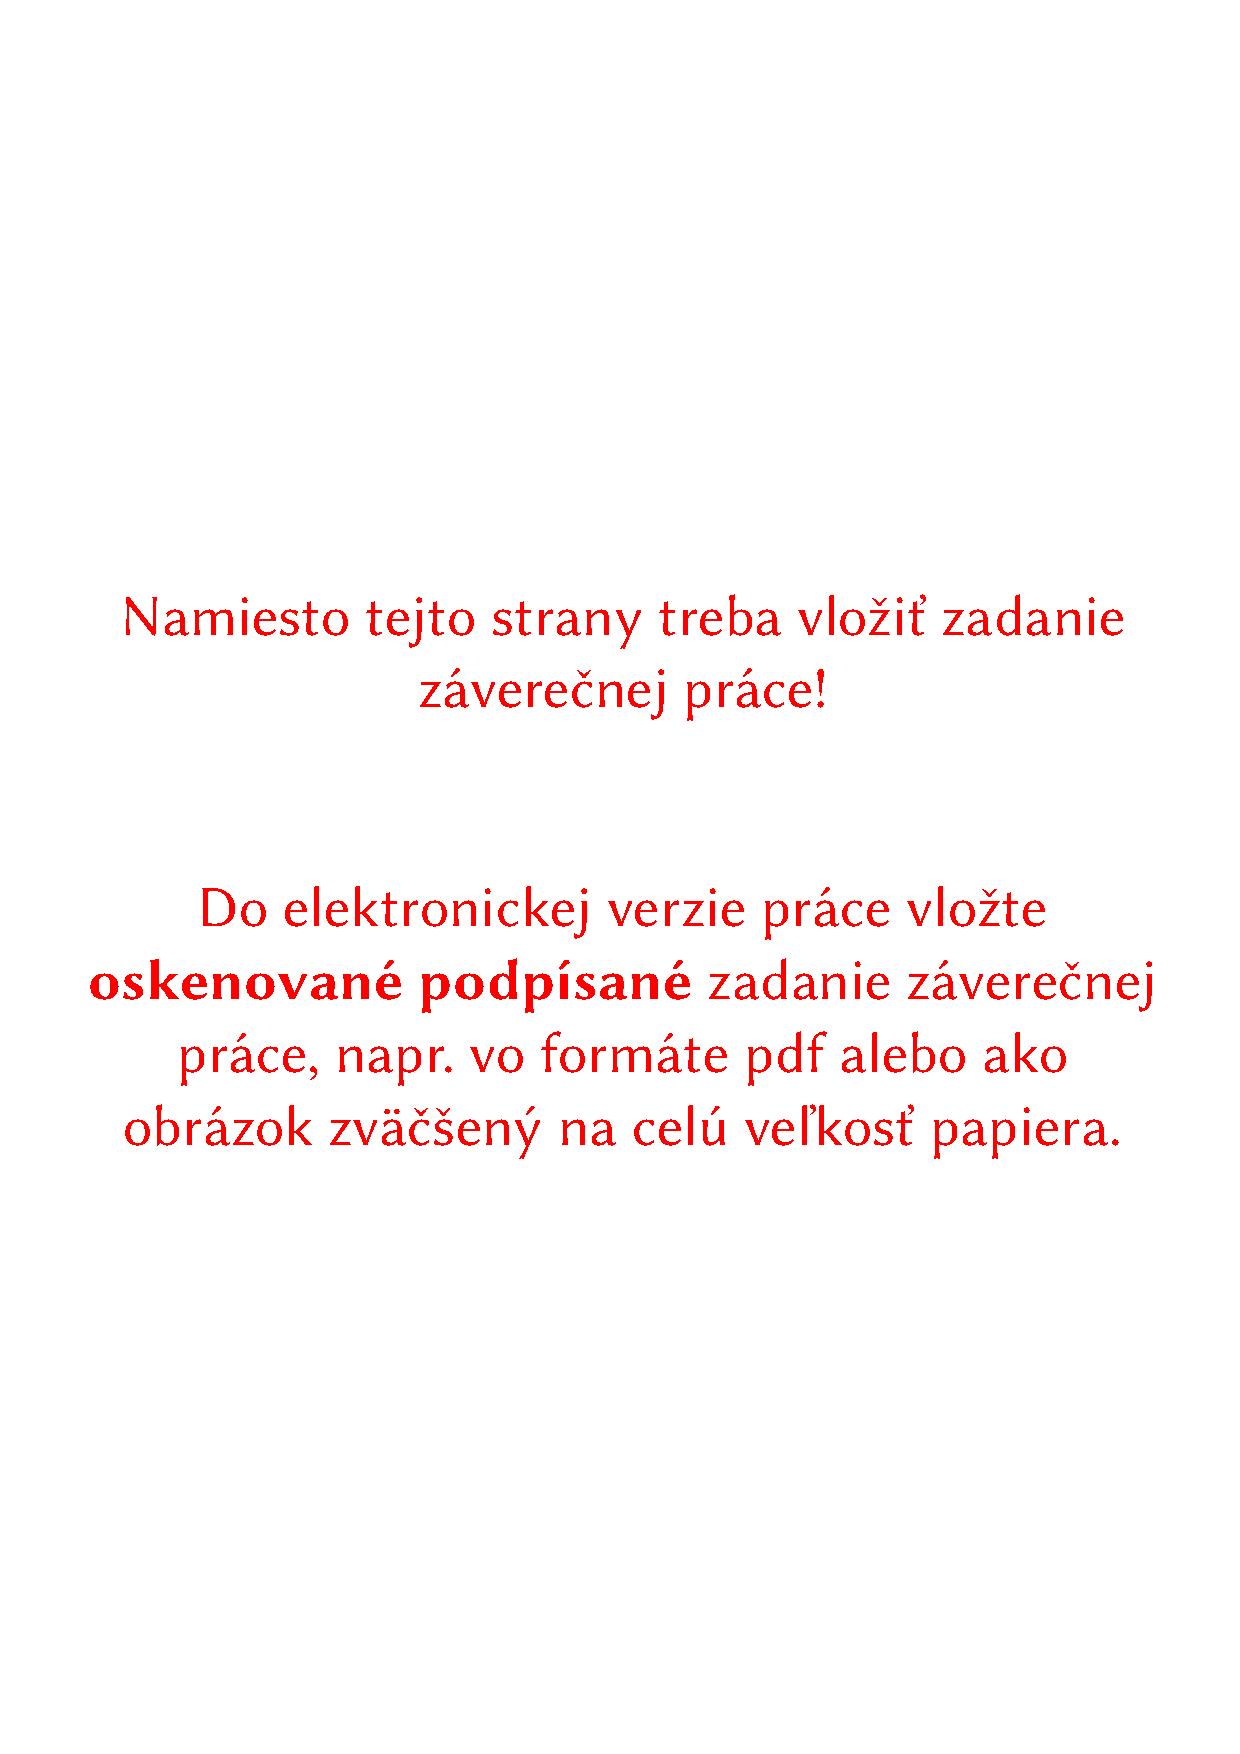
\includepdf[fitpaper]{modules/zadanie.pdf}

%-------------------------------------------------------
%				Front Matter (TOC, LOF, ...)
%-------------------------------------------------------
\frontmatter

% suppress some commands in TOC and lists
\begingroup
\renewcommand{\ac}[1]{#1}
\renewcommand{\cite}[1]{}

% Poďakovanie
\makeacknowledgements

% Abstrakt, anotácia
\makeabstract

%  TOC
\etocdepthtag.toc{mtchapter}
\etocsettagdepth{mtchapter}{subsection}
\etocsettagdepth{mtappendix}{none}
\tableofcontents

% list of figures
\etocdepthtag.toc{mtfigure}
\etocsettagdepth{mtfigure}{subsection}
\etocsettagdepth{mtfigure}{none}
\iftotalfigures\listoffigures\fi

% list of tables
\etocdepthtag.toc{mttable}
\etocsettagdepth{mttable}{subsection}
\etocsettagdepth{mttable}{none}
\iftotaltables\listoftables\fi

% list of abbreviations
\acsetup{page-ref=comma,list-style=acronyms
}{
	\ifargoutempty{\printacronyms[include-classes=abbrev,heading=none]}{}{
		\unchapter{Zoznam skratiek}
		\argoutemptyFirstArg
	}
}

% dictionary
\acsetup{page-ref=none,list-style=dictstyle,extra-style=plain,extra-format={\;},only-used=false}{
\ifargoutempty{\printacronyms[include-classes=dict,heading=none]}{}{
	\unchapter{Slovník pojmov}
	\setlength{\columnseprule}{0.2pt}
	\setlength{\columnsep}{1.25cm}
	\begin{multicols}{2}
	\argoutemptyFirstArg
	\end{multicols}
}}

\endgroup % suppress some commands in TOC and lists

%-------------------------------------------------------
%						Document
%-------------------------------------------------------
\mainmatter

% !TeX spellcheck = sk_SK
\chapter{Úvod}

V úvode autor stručne a výstižne charakterizuje stav poznania alebo praxe v oblasti, ktorá je predmetom záverečnej práce a oboznamuje čitateľa s významom, cieľmi a zámermi práce. Autor v úvode zdôrazňuje, prečo je práca dôležitá a prečo sa rozhodol spracovať danú tému.

% !TeX spellcheck = sk_SK
\chapter{Postup práce so šablónou}

Šablóna pre LaTeX obsahuje všetko potrebné na vygenerovanie PDF verzie záverečnej práce v predpísanom formáte. Ako ju teda použiť? Všetky základné informácie potrebné na prácu s ňou predstavíme v tejto kapitole. Diskusiu začneme tým, ako je šablóna štruktúrovaná. Potom zhrnieme ako vyplniť potrebné metadáta o dokumente a ako písať obsah jadra práce. Následne prejdeme k tomu, aké softvérové prostredie je potrebné, aby sme dokázali prácu skompilovať do podoby finálneho PDF dokumentu.

\section{Štruktúra šablóny}

Dokumenty pre LaTeX sa skladajú z viacerých súborov, ktoré nie sú zabalené do jedného archívu ako to býva pri dokumentoch pre Microsoft Word, LibreOffice alebo pre podobné softvérové produkty. Podobajú sa viac na zdrojové kódy programu než na klasický dokument.

Naša šablóna má nasledujúcu štruktúru:
\begin{itemize}
\item Súbor \textbf{\texttt{main.tex}} je hlavným súborom šablóny. Definujú sa v ňom základné metadáta dokumentu a include-ujú sa z neho súbory jednotlivých kapitol.

\item Jednotlivé kapitoly dokumentu sú v osobitných súboroch. Názvy súborov u nás začínajú predponou \textbf{\texttt{kap\_}} -- čisto kvôli prehľadnosti.

\item Bibliografické údaje o citovaných publikáciách sú v špeciálnom BibTeX súbore s názvom \textbf{\texttt{bibliography.bib}}.

\item Súbory \textbf{\texttt{iso.bbx}}, \textbf{\texttt{iso-fullcite.cbx}}, \textbf{\texttt{iso-numeric.bbx}}, \textbf{\texttt{iso-numeric.cbx}} a\ \textbf{\texttt{slovak.lbx}} definujú citačný štýl.

\item Súbor \textbf{\texttt{style.sty}} definuje štýl dokumentu a niektoré pomocné makrá, ktoré používame.

\item Súbor \textbf{\texttt{makepdf.sh}} je pomocný skript, ktorý ukazuje ako možno vykompilovať dokument z príkazového riadku. Vykompilovaný dokument aj pomocné súbory sa kvôli prehľadnosti ukladajú do pomocného priečinka \texttt{auxfiles} -- inak by sa miešali so zdrojovými súbormi.
\end{itemize}

Používame nasledujúce podadresáre:
\begin{itemize}
\item \textbf{\texttt{images}} -- obsahuje obrázky,
\item \textbf{\texttt{listings}} -- obsahuje zdrojové kódy,
\item \textbf{\texttt{modules}} -- obsahuje pomocné súbory, prípadne celé strany, ktoré treba niekam vložiť.
\end{itemize}

Súbor \texttt{modules/abbterms.tex} obsahuje databázu pojmov a skratiek -- viac informácií o ňom možno nájsť v časti \ref{sec:skratky}.

\section{Metadáta o dokumente}

V súbore \texttt{main.tex} sa definujú rôzne metadáta dokumentu -- na prvom mieste meno autora a názov práce, ale aj abstrakt, anotácia, dátum odovzdania práce a pod. Keď sa všetky tieto informácie vyplnia, automaticky sa z nich vygeneruje titulná strana, anotačný záznam atď.

\section{Kompilácia dokumentu}

Pri kompilácii dokumentu môžeme postupovať dvojako -- buď použijeme lokálnu inštaláciu LaTeX-u alebo zvolíme cloudové riešenie a na dokumente budeme pracovať nie lokálne, ale prostredníctvom webového rozhrania. Začnime druhou možnosťou -- keďže tá si nevyžaduje lokálnu inštaláciu žiadneho softvéru.

\subsection{Cloudové riešenie -- služba Overleaf}

Jednou možnosťou pri kompilácii LaTeX-ových dokumentov je použiť cloudové riešenie -- napríklad služby Overleaf: \href{https://www.overleaf.com/}{overleaf.com}. Po registrácii dostane užívateľ k dispozícii priestor kam môže uploadovať svoje dokumenty, pracovať na nich, kompilovať ich do formátu PDF atď. Služba Overleaf umožňuje aj vytváranie rôznych verzií dokumentu a má rozhranie pre git. Hlavnou výhodou cloudového riešenia však je, že lokálne nie je potrebné nič inštalovať. Na druhej strane, naša skúsenosť je, že kompilácia pomocou služby Overleaf trvá pomerne dlho.

\subsubsection{Limitovaný počet súborov}

Jedným dosť nepríjemným obmedzením služby Overleaf (iné analogické služby sú na tom podobne) je limit na počet súborov v projekte. V neplatenej verzii služby je to 50, čo je veľmi nízky počet, ak vezmeme do úvahy, že napríklad každý obrázok je v osobitnom súbore. Aj v najvyššej verzii služby je možné v tom istom projekte mať len 1000 súborov, čo v prípade rozsiahlejších publikácií nemusí ani zďaleka stačiť.

\subsection{Lokálna inštalácia -- balík TeXLive}

Ďalšou možnosťou je použiť lokálnu inštaláciu LaTeX-u. Nevýhodou je, že inštalácie bývajú pomerne veľké a sťahujú sa po jednotlivých balíčkoch, čo zvykne trvať dosť dlho. Výhodou je, že lokálna inštalácia je lepšie konfigurovateľná a neaplikujú sa v nej podobné obmedzenia ako v prípade služby Overleaf -- napr. obmedzenie na počet súborov.

Jednou z populárnych distribúcií LaTeX-u je distribúcia TeX Live. Na Linux-e je ju typicky možné nájsť v balíčkovom systéme. Na Windows-e je možné zase použiť jednoduchý grafický inštalátor, ktorý možno stiahnuť na \href{https://www.tug.org/texlive/}{tug.org/texlive/}.

\section{Encxvlna a správne zalamovanie}

Slovenská typografia je charakteristická jednou mierne excentrickou požiadavkou -- že niektoré predložky a spojky nesmú byť na konci riadku. Ak sa tam vyskytnú, musia sa už zalomiť do nasledujúceho riadku. Na realizáciu tejto funkcionality v LaTeX-u je potrebné použiť balíček \texttt{encxvlna}. Drobná komplikácia spočíva v tom, že tento balíček vyžaduje aktiváciu systému \texttt{enctex}.

V inštalácii TeXLive je možné \texttt{enctex} aktivovať buď pre užívateľa alebo pre celý systém. V oboch prípadoch je na to potrebné vytvoriť súbor s názvom \texttt{fmtutil.cnf}, ktorý bude obsahovať:
\begin{Verbatim}
pdflatex pdftex language.dat -enc -translate-file=cp227.tcx *pdflatex.ini
\end{Verbatim}
Kľúčová je časť \texttt{-enc}, ktorá hovorí, že sa má povoliť \texttt{enctex}.

\subsection{Aktivácia \texttt{enctex}-u pre užívateľa}

V prípade aktivácie pre užívateľa je súbor \texttt{fmtutil.cnf} potrebné umiestniť do domovského adresára užívateľa, na cestu \texttt{texmf/web2c}.

Následne treba z príkazového riadku spustiť príkaz:
\begin{Verbatim}
fmtutil -user --all
\end{Verbatim}
ktorý nanovo prekompiluje užívateľské LaTeX formáty tak, že príkaz pdflatex bude mať aktivovaný \texttt{enctex}.

\subsection{Aktivácia \texttt{enctex}-u pre celý systém}

V prípade aktivácie pre celý systém sa súbor \texttt{fmtutil.cnf} umiestni do adresára LaTeX-ovej inštalácie, na cestu \texttt{texmf-local/web2c}. Následne je znovu potrebné prekompilovať LaTeX formáty, lenže systémové. Používa sa na to príkaz:
\begin{Verbatim}
fmtutil -sys --all
\end{Verbatim}
Keďže príkaz modifikuje systémovú inštaláciu, môže byť potrebné spustiť ho s administrátorskými privilégiami. Napr. na Ubuntu sa to dosiahne pomocou príkazu \texttt{sudo}.

\subsection{Overleaf a \texttt{enctex}}

V systéme Overleaf nie je enctex možné aktivovať -- preto na kompiláciu dokumentu je potrebné zakomentovať riadok \texttt{\textbackslash{usepackage}\{encxvlna\}} v \texttt{main.tex}.

\section{Includeonly}

V prípade rozsiahlejšieho dokumentu môže kompilácia do PDF trvať neprimerane dlho. Preto je užitočné niekedy dokument prestaviť tak, aby sa generovala len nejaká jeho menšia časť -- typicky jedna kapitola. To by však mohlo poškodiť odkazy na iné kapitoly, zmeniť číslovanie strán a pod. -- takže vygenerovaná kapitola by vyzerala inak než bude vyzerať vo finálnom texte.

Preto existuje prostredie \texttt{includeonly}, v rámci ktorého sa dá zadefinovať, z ktorých \texttt{.tex} súborov vložených pomocou makra \texttt{include} sa má aktuálne generovať. Pomocné súbory vygenerované z ostatných \texttt{.tex} súborov sú však stále k dispozícii a preto sa dajú čísla strán, odkazy a všetko ostatné v aktuálnom PDF realizovať korektne -- presne v takom tvare, ako to bude aj vo finálnej verzii.

Prostredie \texttt{includeonly} je už pripravené v súbore \texttt{main.tex} -- stačí ho odkomentovať a vložiť názvy tých súborov, z ktorých sa má aktuálne generovať PDF.

% !TeX spellcheck = sk_SK
\chapter{Základy písania v LaTeX-u}

V tejto časti ukážeme ako sa v LaTeX-u realizujú niektoré základné operácie ako je napr. členenie textu do kapitol a podkapitol, vkladanie obrázkov, tabuliek, rovníc, či listingov zdrojových kódov a pod.

\section{Členenie textu}
\label{sec:clenenie_textu}

Členenie textu na kapitoly, podkapitoly a menšie sekcie sa v LaTeX-u realizuje pomocou nasledujúcich príkazov:
\begin{itemize}
\item \texttt{{\textbackslash}chapter}\{názov\}: nadpis 1. úrovne.
\item \texttt{{\textbackslash}section}\{názov\}: nadpis 2. úrovne.
\item \texttt{{\textbackslash}subsection}\{názov\}: nadpis 3. úrovne.
\item \texttt{{\textbackslash}subsubsection}\{názov\}: nadpis 4. úrovne.
\item \texttt{{\textbackslash}paragraph}\{názov\}: nadpis odseku.
\end{itemize}
Ukážka toho, ako sa jednotlivé typy kapitol zobrazujú, nasleduje nižšie.

\subsection{Subsection}

\blindtext

\subsubsection{Subsubsection}

\blindtext

\paragraph{Paragraph}

\blindtext

\subsection{Odkazy na kapitoly}

Aby sa na kapitoly dalo odkazovať, treba pod nadpis kapitoly vložiť návesť na ňu pomocou makra \texttt{label}, napr.:
\begin{inlinecode}{latex}
\section{Členenie textu}
\label{sec:clenenie_textu}
\end{inlinecode}

Časť \texttt{sec:} nie je povinná -- je však dobrým zvykom návestia označovať podľa toho, na čo odkazujú: napr. \texttt{sec} pre kapitoly, \texttt{fig} pre obrázky, \texttt{eq} pre rovnice a pod.

Samotné odkazy sa potom generujú pomocou makra \texttt{ref} takto:
\begin{inlinecode}{latex}
\ref{sec:clenenie_textu}
\end{inlinecode}

Odkaz na kapitolu o členení textu by teda vyzeral nasledovne: \ref{sec:clenenie_textu}. V PDF verzii dokumentu sú odkazy vybavené aj hypertextovými prepojeniami. Tie sú v texte označené farebnými rámčekmi. V tlačenej verzii sa rámčeky prirodzene nezobrazujú.

\subsection{Skrátené názvy}

V prípade, že názov kapitoly alebo inej sekcie textu je príliš dlhý na to, aby sa korektne zobrazoval povedzme v záhlaví strany alebo v obsahu práce, dá sa okrem hlavného názvu špecifikovať aj skrátený názov, ktorý sa použije práve na tieto účely. Špecifikuje sa pomocou nepovinného parametra, ktorý sa uzatvorí do hranatých zátvoriek, napr.:
\begin{inlinecode}{latex}
\chapter[Skrátený nadpis kapitoly]{Nepríjemne dlhý a ťažko zobraziteľný nadpis kapitoly, ktorý sa naozaj nikam nezmestí bez toho, aby sa mu vyhradila osobitná strana}
\end{inlinecode}

\section{Vkladanie obrázkov}

Vkladanie obrázkov sa dá realizovať pomocou prostredia \texttt{figure} nasledovne:
\begin{inlinecode}{latex}
\begin{figure}
\centering

\includegraphics[width=5cm]{logo}
\caption{Logo elektrotechnickej fakulty.}
\label{fig:obrazok}
\end{figure}
\end{inlinecode}

Výsledok ilustruje \figurename~\ref{fig:obrazok}. Pozícia obrázka sa určí automaticky -- typicky je snaha obrázky umiestniť buď do vrchnej alebo do spodnej časti strany, t.j. nie doprostred textu. V prípade, že to nie je možné (napr. obrázok je príliš veľký), môže byť obrázok umiestnený aj na osobitnú stranu. Umiestnenie obrázkov je možné ovplyvniť použitím nepovinného parametra -- viac o tom je možné pozrieť v návode \cite{latexFigures}.

\begin{figure}
\centering

\includegraphics[width=5cm]{logo}
\caption{Logo elektrotechnickej fakulty.}
\label{fig:obrazok}
\end{figure}

Odkazovanie sa na obrázky sa realizuje pomocou značky uvedenej vo vnútri makra \texttt{label}. V tomto prípade ide o značku \texttt{fig:obrazok}. Odkaz na obrázok zapíšeme teda ako:
\begin{inlinecode}{latex}
\figurename~\ref{fig:obrazok}
\end{inlinecode}
kde makro {\textbackslash}figurename vracia názov popiskov obrázkov v aktuálnom jazyku (u nás je to \figurename) a {\textbackslash}ref{fig:obrazok} generuje samotný odkaz. Vlnovka \textasciitilde\ označuje nezalomiteľnú medzeru.

\subsection{Viacero obrázkov vedľa seba}

Niekedy -- ak jednotlivé obrázky nezaberajú priveľa miesta -- je užitočné uložiť ich aj viacero vedľa seba. Dá sa to docieliť pomocou prostredia \texttt{minipage} napríklad nasledovne:
\begin{inlinecode}{latex}
\begin{figure}
\centering
\begin{minipage}[b]{0.58\textwidth}
\centering
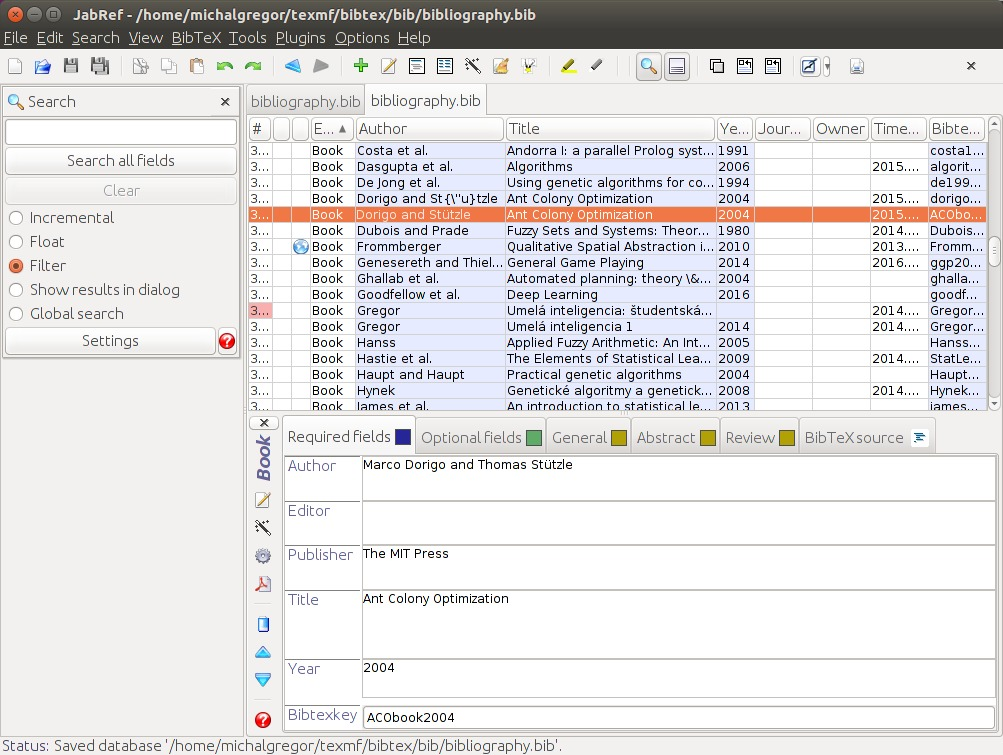
\includegraphics[width=\textwidth]{jabref}
\caption{Prvý obrázok.}
\label{fig:mini1}
\end{minipage}\quad
\begin{minipage}[b]{0.38\textwidth}
\centering

\includegraphics[width=\textwidth]{logo}
\caption{Druhý obrázok.}
\label{fig:mini2}
\end{minipage}
\end{figure}
\end{inlinecode}

Výsledkom je viacero obrázkov uložených vedľa seba, ako to ukazujú \figurename~\ref{fig:mini1} a \figurename~\ref{fig:mini2}.

\begin{figure}
\centering
\begin{minipage}[b]{0.58\textwidth}
\centering
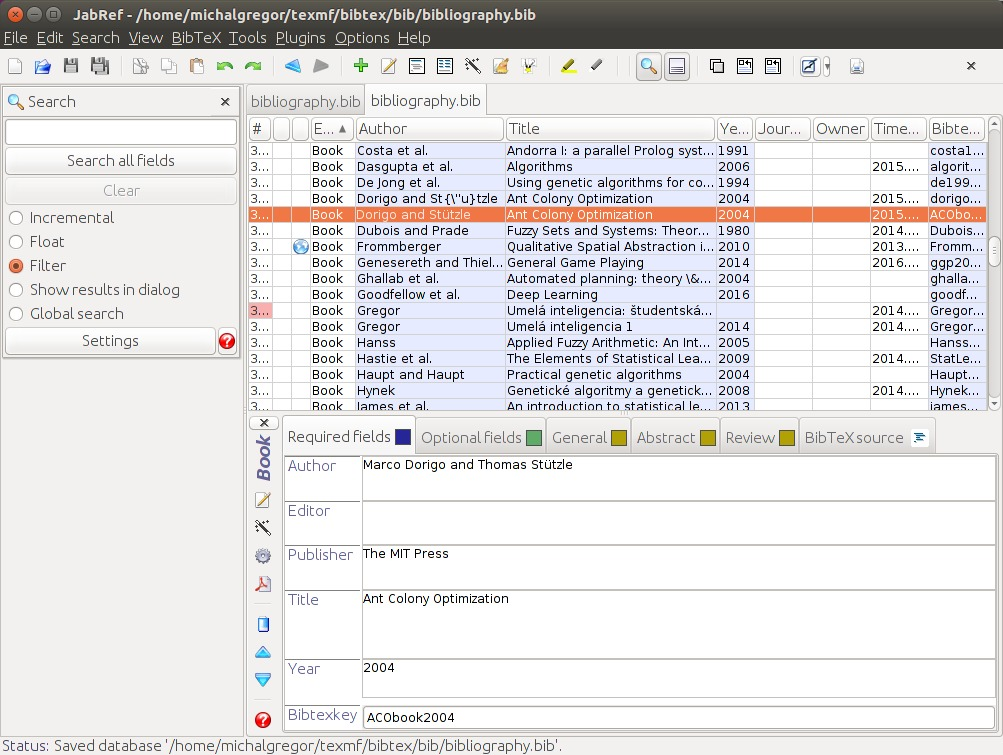
\includegraphics[width=\textwidth]{jabref}
\caption{Prvý obrázok.}
\label{fig:mini1}
\end{minipage}\quad
\begin{minipage}[b]{0.38\textwidth}
\centering

\includegraphics[width=\textwidth]{logo}
\caption{Druhý obrázok.}
\label{fig:mini2}
\end{minipage}
\end{figure}

Ako vidno, do toho istého \texttt{figure} prostredia sme vložili dve \texttt{minipage} prostredia -- jedno pre každý obrázok. Povinným argumentom \texttt{minipage} prostredia je jeho šírka -- časť strany sme nechali jednému a časť druhému obrázku a nejaké miesto sme vynechali aj pre medzeru medzi nimi. Nepovinným argumentom, ktorý sa uvádza v hranatých zátvorkách, je ako majú byť obrázky voči sebe vertikálne zarovnané. My sme zvolili možnosť \texttt{[b]}, t.j. majú byť zarovnané spodnou časťou.

\subsection{Podobrázky}

Obdobným spôsobom sa dajú vkladať podobrázky -- ibaže namiesto prostredia \texttt{minipage} sa použije prostredie \texttt{subfigure}. Príklad nasleduje tu:
\begin{inlinecode}{latex}
\begin{figure}
\centering
\begin{subfigure}[c]{0.5\textwidth}
	\centering
	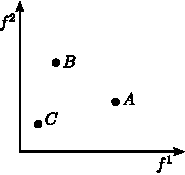
\includegraphics[width=6.5cm]{pareto_dominance}
	\caption{Pareto dominancia.}
	\label{fig:subfig1}
\end{subfigure}~
\begin{subfigure}[c]{0.5\textwidth}
	\centering
	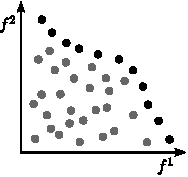
\includegraphics[width=6.5cm]{pareto_front}
	\caption{Pareto front.}
	\label{fig:subfig2}
\end{subfigure}
\caption{Ilustrácia: Pareto dominancia a Pareto front.}
\label{fig:fig_with_subfigs}
\end{figure}
\end{inlinecode}

Ako vidno na \figurename~\ref{fig:fig_with_subfigs}, obrázok má jeden spoločný popisok a takisto každý z podobrázkov má popisok, na ktorý sa dá odkazovať, napr. \figurename~\ref{fig:subfig1}.

\begin{figure}
\centering
\begin{subfigure}[c]{0.5\textwidth}
	\centering
	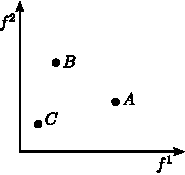
\includegraphics[width=6.5cm]{pareto_dominance}
	\caption{Pareto dominancia.}
	\label{fig:subfig1}
\end{subfigure}~
\begin{subfigure}[c]{0.5\textwidth}
	\centering
	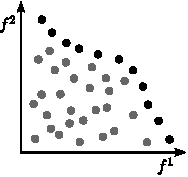
\includegraphics[width=6.5cm]{pareto_front}
	\caption{Pareto front.}
	\label{fig:subfig2}
\end{subfigure}
\caption{Ilustrácia: Pareto dominancia a Pareto front.}
\label{fig:fig_with_subfigs}
\end{figure}

\subsection{Vektorové a rastrové obrázky}

Vkladané obrázky by -- podľa možnosti -- mali mať vektorový formát. Platí to najmä v prípade schém, diagramov a pod. Rastrový formát obrázkov je prípustný v prípade, že ide o fotografie, screenshot-y alebo iné typy obrazového materiálu, ktoré majú prirodzene rastrovú formu. Rastrová forma je takisto vhodná v prípade nadštandardne zložitých obrázkov, ktorých vykresľovanie z vektorového formátu by pri zobrazovaní trvalo príliš dlho.

Najvhodnejšie formáty obrázkov pri použití v LaTeX-u sú zrejme \texttt{eps} a \texttt{pdf}. Existuje viacero dobrých nástrojov na tvorbu kvalitných vektorových obrázkov. Zdarma je k dispozícii napríklad nástroj Inkscape: \href{https://inkscape.org/en/}{inkscape.org}. Na editovanie rastrových obrázkov je zase možné použiť napríklad GIMP: \href{https://www.gimp.org/}{gimp.org}.

\subsection{Obrázky obtekané textom}

V odborných prácach sa spravidla nepoužívajú obrázky obtekané textom -- ich používanie neodporúčame ani v záverečnej práci. Navyše v LaTeX-u sa obtekanie dosahuje pomocou prostredia \texttt{wrapfigure}, ktoré je málo robustné a často spôsobuje nesprávne zalomenie textu a pod.

\subsection{Obrázky v landscape režime}

V prípade, že je potrebné vložiť obzvlášť veľký a široký obrázok (ktorý by nebol dostatočne čitateľný v zmenšenej podobe), je možné zobraziť ho na osobitnej strane v landscape režime. Používa sa na to prostredie \texttt{sidewaysfigure}, napr.:
\begin{inlinecode}{latex}
\begin{sidewaysfigure}[p]
\centering
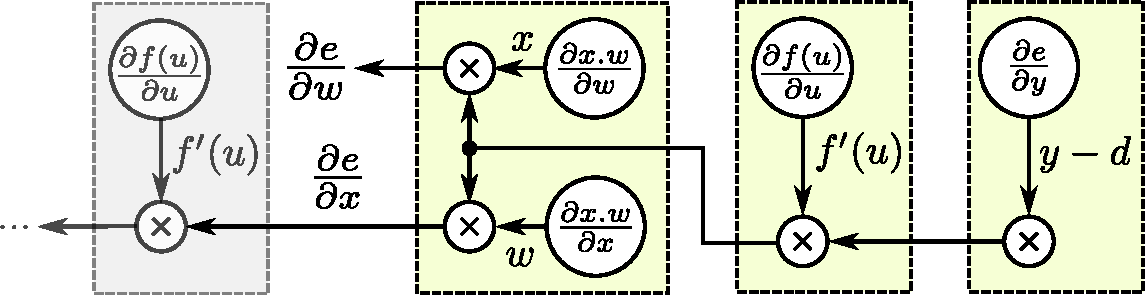
\includegraphics[width=23cm]{wide_figure}
\caption{Obzvlášť veľký a široký obrázok.}
\end{sidewaysfigure}
\end{inlinecode}

Výsledok vidno na \figurename~\ref{fig:wide_figure}. Pre tabuľky existuje obdobné prostredie \texttt{sidewaystable}.


\subsection{Zachovanie polohy obrázku}

Niekedy je potrebné zabezpečiť aby sa obrázok v texte zobrazil na predom určenom mieste, napr. medzi dvoma časťami práce, ktoré s ním súvisia. Niektoré možnosti polohovania obrázka sú napr.: na mieste kde sa nachádza v zdrojovom kóde \texttt{[h]}, na vrchnej \texttt{[t]} alebo na spodnej \texttt{[b]} časti strany. 

Toto je text, ktorý súvisí s \figurename~\ref{fig:obrazok2} nižšie.

\begin{figure}[h]
\centering

\includegraphics[width=5cm]{logo}
\caption{Logo elektrotechnickej fakulty.}
\label{fig:obrazok2}
\end{figure}

Toto je text, ktorý súvisí s \figurename~\ref{fig:obrazok2} vyššie. Umiestnenie obrázka bolo dosiahnuté pomocou:

\begin{inlinecode}{latex}
\begin{figure}[h]
\centering

\includegraphics[width=5cm]{logo}
\caption{Logo elektrotechnickej fakulty.}
\label{fig:obrazok2}
\end{figure}
\end{inlinecode}

\begin{sidewaysfigure}[p]
\centering
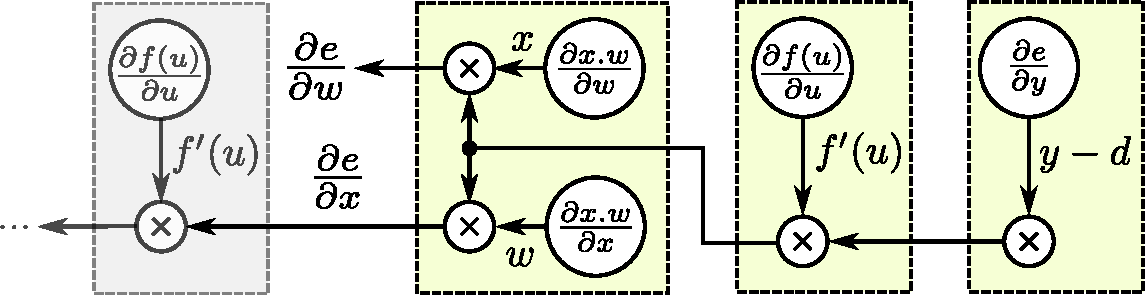
\includegraphics[width=23cm]{wide_figure}
\caption{Obzvlášť veľký a široký obrázok.}
\label{fig:wide_figure}
\end{sidewaysfigure}


\section{Tabuľky}

Ďalší prvok, ktorý bude obsahovať väčšina záverečných prác, sú tabuľky. Vzhľadom na to, že tvorba tabuliek v LaTeX-u je pomerne komplikovaná, nebudeme sa na tomto mieste zaoberať všetkými detailami -- uvedieme len niekoľko základných ukážok. Iné príklady je možné nájsť povedzme v \cite{latexTables}.

Začnime jednoduchým príkladom: \tablename~\ref{tab:priklad}. Túto tabuľku je možné vygenerovať pomocou nasledujúceho kódu:
\begin{inlinecode}{latex}
\begin{table}
\centering
\caption{Príklad jednoduchej tabuľky.}
\label{tab:priklad}
\begin{tabular}{|l|c|r|}
\hline
\textbf{č. 1} & \textbf{č. 2} &  \textbf{č. 3} \\
\hline
1 & 2 & 3 \\
11 & 22 & 33 \\
111 & 222 & 333 \\
\hline
\end{tabular}
\end{table}
\end{inlinecode}
Odkaz na tabuľku sa píše v tvare:
\begin{inlinecode}{latex}
\tablename~\ref{tab:priklad}
\end{inlinecode}

Ako vidno, celá tabuľka je obalená do prostredia \texttt{table}. Toto prostredie je plávajúce -- čiže podobne ako v prípade obrázkov sa mu pozícia určuje automaticky. Samotné jadro tabuľky sa tvorí pomocou prostredia \texttt{tabular}. Jeho prvým argumentom je formátovanie stĺpcov. Pre každý stĺpec tabuľky tu vystupuje jedno písmenko, ktoré určuje zarovnanie (\texttt{l} -- doľava, \texttt{c} -- na stred, \texttt{r} -- doprava). Zvislé čiary medzi stĺpcami znamenajú zvislé orámovanie.

\begin{table}
\centering
\caption{Príklad jednoduchej tabuľky.}
\label{tab:priklad}
\begin{tabular}{|l|c|r|}
\hline
\textbf{č. 1} & \textbf{č. 2} &  \textbf{č. 3} \\
\hline
1 & 2 & 3 \\
11 & 22 & 33 \\
111 & 222 & 333 \\
\hline
\end{tabular}
\end{table}

Samotné riadky tabuľky sa vpisujú do vnútra prostredia \texttt{tabular}. Jednotlivé bunky sú od seba oddelené ampersandmi \& a každý riadok je ukončený značkou \textbackslash\textbackslash. Horizontálne orámovanie sa dá vložiť pomocou príkazu \texttt{{\textbackslash}hline}.

%TODO: Viac ku tabuľkám.

%\subsection{Horizontálne zlučovanie buniek}
%
%
%
%\subsection{Vertikálne zlučovanie buniek}
%
%
%
%\subsection{Lomené bunky}
%
%
%
%\subsection{Dlhé tabuľky}
%
%
%\todo[inline]{Dokončiť; pridať aj zložitejšie príklady s lomenými bunkami, krajšie formátovanými tabuľkami, multirow a multicol prípadmi a pod. longtable}


\section{Zoznam obrázkov a tabuliek}

Zoznam obrázkov a tabuliek sa v našej šablóne generuje automaticky. Obsahuje len obrázky/tabuľky, ktoré majú popisky. Vygeneruje sa len v tom prípade, že dokument naozaj nejaký obrázok/tabuľku obsahuje.

\section{Skratky a slovník pojmov}
\label{sec:skratky}

Práca má obsahovať zoznam skratiek a (nepovinne) slovník pojmov. Oba sa dajú generovať automaticky. Význam skratky sa najprv definuje v súbore \texttt{modules/abbterms.tex}. V texte sa skratka následne obalí do makra \texttt{ac}. Výsledkom je, že každá označená skratka obsahuje hypertextový odkaz na svoju definíciu v zozname skratiek a takisto, že do zoznamu skratiek pribudne číslo strany, na ktorej sa skratka použila.

Zmysel skratky je okrem toho potrebné vysvetliť v texte na tom mieste, kde sa prvýkrát používa -- nestačí len uviesť vysvetlenie v zozname skratiek. Napr. pri prvom použití povieme: umelá neurónová sieť (\angl{artificial neural network}; \ac{ANN}). Pri ďalšom použití stačí už len \ac{ANN}.

Obsah slovníka pojmov sa takisto vypĺňa v súbore \texttt{modules/abbterms.tex}, ale na pojmy sa nie je potrebné odkazovať z textu. V slovníku budú automaticky všetky zadefinované pojmy.

\section{Rovnice}

LaTeX má osobitne dobrú podporu pre sádzanie matematických výrazov, vkladanie rovníc s automatickým číslovaním a pod. Vkladanie rovníc je veľmi jednoduché a rýchle -- akonáhle sa užívateľ naučí základy syntaxe, ktorá je potrebná na ich zápis.

Matematické symboly a vzorce, ktoré majú byť súčasťou bežného textu sa označujú párom dolárov a zobrazujú sa nasledovne: $x^2 + \alpha$. Tento odsek by sa teda dal zapísať nasledujúcim spôsobom:
\begin{inlinecode}{latex}
Matematické symboly a vzorce, ktoré majú byť súčasťou bežného
textu sa označujú párom dolárov a zobrazujú sa nasledovne: $x^2 + \alpha$.
Tento odsek by sa teda dal zapísať nasledujúcim spôsobom:
\end{inlinecode}

Rovnice, ktoré sa majú zobrazovať osobitne, mimo riadku a majú byť číslované, sa dajú vložiť pomocou prostredia \texttt{equation}. Vyzerajú nasledovne:
\begin{equation}
x^2 + \alpha,
\label{eq:dolezita_rovnica}
\end{equation}
kde $x$ je premenná a $\alpha$ je konštanta.

Ak do rovnice vložíme návestie pomocou príkazu \texttt{label}, napr.:
\begin{inlinecode}{latex}
\begin{equation}
x^2 + \alpha,
\label{eq:dolezita_rovnica}
\end{equation}
\end{inlinecode}
môžeme sa na rovnicu odkázať z textu pomocou príkazu \texttt{{\textbackslash}eqref}, t.j.:
\begin{inlinecode}{latex}
Odkaz na rovnicu \eqref{eq:dolezita_rovnica} z textu.
\end{inlinecode}

Výsledný odkaz sa zobrazí nasledovne: Odkaz na rovnicu \eqref{eq:dolezita_rovnica} z textu.

\subsection{Odseky pokračujúce za rovnicou}

Všimnite si, že text nasledujúci za rovnicou nie je odsadený. Nejde totiž o nový odsek, ale o pokračovanie predošlého odseku -- dokonca o pokračovanie tej istej vety. Ak má LaTeX text interpretovať takto, nesmie sa za prostredím equation vynechať nový riadok, t.j. kód bude vyzerať takto:
\begin{inlinecode}{latex}
Rovnice, ktoré sa majú zobrazovať osobitne, mimo riadku a majú byť číslované, sa dajú vložiť pomocou prostredia \texttt{equation}. Vyzerajú nasledovne:
\begin{equation}
x^2 + \alpha,
\end{equation}
kde $x$ je premenná a $\alpha$ je konštanta.
\end{inlinecode}

Keby sa nový riadok vynechal, bude LaTeX text za rovnicou interpretovať už ako nový odsek a výsledok bude nasledovný:
\begin{equation}
x^2 + \alpha,
\end{equation}
% tento prázdny riadok je tu úmyselne
	
kde $x$ je premenná a $\alpha$ je konštanta.

\subsection{Viacero rovníc pod sebou}

LaTeX poskytuje aj dobré nástroje na zobrazovanie viacerých rovníc pod sebou. Je ich možné zobraziť buď centrované -- pomocou prostredia \texttt{gather} -- alebo zarovnané -- pomocou prostredia \texttt{align}.

Centrované rovnice môžu vyzerať nasledovne:
\begin{gather}
x = 2a - 3b \\
y = x^2.
\end{gather}

Kód potrebný na ich zobrazenie vyzerá takto:
\begin{inlinecode}{latex}
\begin{gather}
x = 2a - 3b \\
y = x^2.
\end{gather}
\end{inlinecode}

Zarovnané rovnice môžu zase vyzerať napríklad takto:
\begin{align}
x &= 2a - 3b \\
y &= x^2.
\end{align}

Kód potrebný na ich zobrazenie vyzerá nasledovne:
\begin{inlinecode}{latex}
\begin{align}
x &= 2a - 3b \\
y &= x^2.
\end{align}
\end{inlinecode}

Alternatívne sa dajú použiť prostredia \texttt{gathered} a \texttt{aligned} -- ide o alternatívy, ktoré sa používajú zvnútra prostredia \texttt{equation}. Rovnica sa potom správa ako jeden celok a má len jedno spoločné číslovanie. Číslovanie sa dá potlačiť pre jednotlivé riadky rovnice aj použitím makra \texttt{{\textbackslash}notag}.

\section{Úvodzovky}

Vzhľadom na to, že v každom jazyku sa úvodzovky zapisujú trochu inak, obsahuje LaTeX makro \texttt{enquote} (z balíčka \texttt{csquotes}), ktoré správnu formu úvodzoviek pre daný jazyk generuje. Text, ktorý má byť v úvodzovkách sa teda obalí do makra \texttt{enquote} takto:
\begin{inlinecode}{latex}
\enquote{Text v úvodzovkách}
\end{inlinecode}

Výsledok môže vyzerať napríklad nasledovne: \enquote{Text v úvodzovkách}. Úvodzovky majú viacero úrovní, takže makro \texttt{enquote} môže byť aj vnorené, napr.: \enquote{Text vo vonkajších úvodzovkách, \enquote{text vo vnútorných úvodzovkách}.}

Mnohé LaTeX-ové editory majú pre \texttt{enquote} vstavanú podporu, takže priamo pri písaní vkladajú namiesto úvodzoviek rovno toto makro.

\section{Zoznamy}

Ďalej treba vedieť, ako sa v LaTeX-u zapisujú zoznamy. Existuje ich niekoľko typov -- na prvom mieste ide o číslované a nečíslované zoznamy -- ale v tejto podkapitole sa pozrieme aj na niektoré ďalšie.

\subsection{Číslované zoznamy}

Číslované zoznamy sa vytvárajú pomocou prostredia \texttt{enumerate}, napr.:
\begin{inlinecode}{latex}
\begin{enumerate}
\item položka,
\item položka,
\item položka.
\end{enumerate}
\end{inlinecode}

Zoznam sa zobrazí nasledovne:
\begin{enumerate}
\item položka,
\item položka,
\item položka.
\end{enumerate}

\subsection{Nečíslované zoznamy}

Úplne obdobne sa vytvárajú nečíslované zoznamy -- ibaže sa použije prostredie \texttt{itemize}. Výsledok môže vyzerať nasledovne:
\begin{itemize}
\item položka,
\item položka,
\item položka.
\end{itemize}

\subsection{Viacstĺpcové zoznamy}

V prípade, že zoznam obsahuje viacero položiek, ktoré v horizontálnom smere nezaberajú veľa miesta, môže byť lepšie usporiadať ich do viacerých stĺpcov. V tom prípade sa dá celý zoznam obaliť do prostredia \texttt{multicols} nasledujúcim spôsobom:
\begin{inlinecode}{latex}
\begin{multicols}{2}
\begin{itemize}
\item položka,
\item položka,
\item položka,
\item položka,
\item položka,
\item položka.
\end{itemize}
\end{multicols}
\end{inlinecode}

Výsledný zoznam bude mať teraz dva stĺpce:
\begin{multicols}{2}
\begin{itemize}
\item položka,
\item položka,
\item položka,
\item položka,
\item položka,
\item položka.
\end{itemize}
\end{multicols}

\subsection{Inline zoznamy}

V rámci šablóny definujeme aj zoznam \texttt{inlinelist}, ktorý sa zobrazuje inline -- t.j. vo vnútri riadku, napr.:
\begin{inlinelist}
\item položka,
\item položka,
\item položka.
\end{inlinelist}

\section{Poznámky pod čiarou}

Poznámky pod čiarou možno vložiť pomocou príkazu \texttt{footnote}, napr.\footnote{Poznámka pod čiarou.}:
\begin{inlinecode}{latex}
\footnote{Poznámka pod čiarou.}
\end{inlinecode}

Eventuálne je možné pomocou príkazu \texttt{footnotemark} označiť miesto, ku ktorému poznámka patrí a nižšie pomocou príkazu \texttt{footnotetext} definovať jej obsah -- to je užitočné najmä v prípade dlhších poznámok.

\section{Algoritmy}

Algoritmy je možné do práce vkladať buď v podobe pseudokódu, v podobe vývojového diagramu alebo v podobe konkrétneho zdrojového kódu. Vývojové diagramy sa prirodzene vkladajú ako klasické obrázky. Zvyšnými dvomi typmi zobrazenia sa budeme zaoberať v tejto podkapitole.

\subsection{Pseudokód}

Začneme pseudokódom. Pre LaTeX existuje viacero balíčkov na sádzanie pseudokódov. Dobré výsledky možno dosiahnuť napr. pomocou balíčka \texttt{algorithm2e}, ktorý je už include-ovaný do šablóny. Pseudokód možno pomocou neho zapísať napríklad nasledovne:
\begin{inlinecode}{text}
\begin{algorithm}
Zvoliť počiatočné hodnoty pre parametre: $a_0$, $c_0$\;
\For{$k = 1 \text{ až } pocet\_krokov$}{

$\Delta_a \leftarrow 0$; $\Delta_c \leftarrow 0$\;

\ForEach{$(x, d) \in P$}{
	$\Delta_a \leftarrow \Delta_a - \gamma
	\frac{\partial E(x, d, a_{k-1}, c_{k-1})}{\partial a}$\; 
	$\Delta_c \leftarrow \Delta_c - \gamma
	\frac{\partial E(x, d, a_{k-1}, c_{k-1})}{\partial c}$\;
}

$a_{k} = a_{k-1} + \Delta_a$\;
$c_{k} = c_{k-1} + \Delta_c$\;
}
\caption{Príklad pseudokódu.}
\label{alg:graddesc_iterative}
\end{algorithm}
\end{inlinecode}
Výsledný pseudokód ukazuje \algorithmname~\ref{alg:pseducode}. Na pseudokódy sa odkazujeme pomocou kódu v tvare \texttt{{\textbackslash}algorithmname\textasciitilde{\textbackslash}ref\{alg:pseducode\}}.

\begin{algorithm}
Zvoliť počiatočné hodnoty pre parametre: $a_0$, $c_0$\;
\For{$k = 1 \text{ až } pocet\_krokov$}{

$\Delta_a \leftarrow 0$; $\Delta_c \leftarrow 0$\;

\ForEach{$(x, d) \in P$}{
	$\Delta_a \leftarrow \Delta_a - \gamma \frac{\partial E(x, d, a_{k-1}, c_{k-1})}{\partial a}$\; 
	$\Delta_c \leftarrow \Delta_c - \gamma \frac{\partial E(x, d, a_{k-1}, c_{k-1})}{\partial c}$\;
}

$a_{k} = a_{k-1} + \Delta_a$\;
$c_{k} = c_{k-1} + \Delta_c$\;
}
\caption{Príklad pseudokódu.}
\label{alg:pseducode}
\end{algorithm}

\subsection{Zdrojový kód}

Ak chceme vložiť zdrojový kód priamo, dá sa použiť prostredie \texttt{code} alebo \texttt{inlinecode} vstavané do šablóny. Ak vkladáme kratší zdrojový kód, ktorý nie je uložený v osobitnom súbore, ale ho budeme písať priamo do dokumentu, použijeme prostredie \texttt{inlinecode}, napr.:
\begin{Verbatim}
\begin{inlinecode}[label={lst:inline_code},
caption={Príklad krátkeho zdrojového kódu.}]{python}
def power(x):
	return x ** 2
\end{inlinecode}
\end{Verbatim}
Ako vidno, aby sa správne zvýraznila syntax, je potrebné zadať, v akom jazyku je kód napísaný. Ak sa syntax zvýrazňovať nemá, namiesto označenia jazyka sa napíše \texttt{text}. Argumenty v hranatých zátvorkách sú nepovinné. Ak zdrojový kód nemá mať titulok, stačí jednoducho vynechať nepovinný parameter \texttt{caption}.

Zdrojový kód sa zobrazí ako to vidno na \listingname~\ref{lst:inline_code}. Na zdrojové kódy sa odkazujeme pomocou zápisu v tvare \texttt{{\textbackslash}listingname\textasciitilde{\textbackslash}inline\_code}.

\begin{inlinecode}[label={lst:inline_code},
caption={Príklad krátkeho zdrojového kódu.}]{python}
def power(x):
	return x ** 2
\end{inlinecode}
Naopak pre prípad dlhších zdrojových kódov, ktoré sú uložené v osobitných súboroch, možno použiť prostredie \texttt{code}, napr.:
\begin{Verbatim}
\begin{code}
\caption{Ukážka dlhšieho zdrojového kódu.}
\inputcode[firstline=5,lastline=39]{python}
	{listings/delta_rule.py}
\label{lst:delta_rule}
\end{code}
\end{Verbatim}

Parametre uvedené v hranatých zátvorkách sú znovu nepovinné -- \texttt{firstline} a \texttt{lastline} určujú, aký rozsah riadkov sa má zobraziť. Ukážka výsledku je na \listingname~\ref{lst:delta_rule}.
\begin{code}
\caption{Ukážka dlhšieho zdrojového kódu.}
\inputcode[firstline=5,lastline=38]{python}
	{listings/delta_rule.py}
\label{lst:delta_rule}
\end{code}
Ak sa zo zdrojového kódu zobrazujú len niektoré riadky, treba pri prípadnom neskoršom editovaní kódu samozrejme dbať na to, aby sa riadky nepoposúvali.

\section{TODO poznámky}

Pri písaní záverečnej práce môže byť užitočné vložiť na niektoré rozpracované miesta TODO poznámky. Dá sa to realizovať pomocou príkazu \texttt{todo}, napr.:
\begin{inlinecode}{latex}
\todo[inline]{Príklad TODO poznámky.}
\end{inlinecode}

\todo[inline]{Príklad TODO poznámky.}

% !TeX spellcheck = sk_SK
\chapter{Ako citovať}

Bibliografické informácie pre LaTeX sa ukladajú vo zvláštnom formáte BibTeX -- v súboroch s príponou \texttt{.bib}. Po každej zmene tohto súboru je potrebné uskutočniť kompiláciu pomocou nástroja Biber aby sa zmeny prejavili. Ukážka BibTeX záznamu pre knihu \enquote{Genetické algoritmy a genetické programování} nasleduje tu:

\begin{inlinecode}{text}
@Book{Hynek2008,
  Title                    = {Genetické algoritmy a genetické programování},
  Author                   = {Josef Hynek},
  Publisher                = {Grada Publishing, a.s.},
  Year                     = {2008},
  Address                  = {Praha},
  ISBN                     = {978-80-7300-218-3}
}
\end{inlinecode}

\section{Príkaz \texttt{cite}}

Keď už ku danej publikácii existuje záznam, citovať ho je veľmi jednoduché -- stačí jeho identifikátor (v tomto prípade \texttt{Hynek2008}) obaliť do makra \texttt{cite}, t.j. \texttt{{\textbackslash}cite\{Hynek2008\}}. Výsledkom je citácia, ktorá sa môže podobať nasledujúcej: \cite{Hynek2008}.

Všimnite si, že citácia je \textbf{vždy súčasťou vety} -- píše sa ešte \textbf{pred bodkou}. V niektorých citačných štýloch sa citácie uvádzajú aj mimo vety/odseku, ale v našom odbore to nie je zvykom.

Do toho istého makra \texttt{cite} sa dá zapísať aj viacero identifikátorov oddelených čiarkami, napr. \texttt{{\textbackslash}cite\{Hynek2008,jabref\}}. V tom prípade vznikne hromadná citácia viacerých zdrojov: \cite{Hynek2008,jabref}.

Citácie sa dajú naopak realizovať aj podrobnejšie. Ak je napríklad žiaduce citovať konkrétnu kapitolu alebo stranu z diela, dá sa na to použiť nepovinný parameter príkazu \texttt{cite}, napr. \texttt{{\textbackslash}cite[s. 125]\{Hynek2008\}}. Výsledná citácia bude vyzerať takto: \cite[s. 125]{Hynek2008}. Takéto podrobné citácie sa však v našej odbornej oblasti prakticky vôbec nepoužívajú -- v drvivej väčšine prípadov je úplne postačujúce citovať pôvodné dielo ako celok.

\section{Parafrázy a doslovné citácie}

Doslovné citácie sa v našom odbore používajú pomerne zriedkavo. Keď hovoríme o citáciách, typicky máme na mysli nie doslovné citácie, ale parafrázy. V prípade parafráz autor práce píše text vlastnými slovami a citácie uvádza len ako zdroj, odkiaľ čerpá informácie.

Ak autor cituje doslova -- t.j. preberá konkrétne znenie textu z pôvodného zdroja -- musí citáciu viditeľne oddeliť od ostatného textu. Pri kratších úsekoch textu sa citácia označí úvodzovkami, napr.: \enquote{Genetické algoritmy sa často využívajú na riešenie rozmanitých optimalizačných úloh...} \cite{Hynek2008}.

Ak sa doslovne preberá dlhší úsek textu, napr. celý odsek alebo niekoľko odsekov, používajú sa blokové citácie, napr. \cite{Hynek2008}:
\begin{quotation}
Genetické algoritmy sa často využívajú na riešenie rozmanitých optimalizačných úloh, ale hádam ešte častejšie sa jednoduché extremálne úlohy využívajú na názorné predvedenie ich ľahkej aplikovateľnosti a funkčnosti. Aj konkrétny problém, na ktorý bude aplikovaný genetický algoritmus v tejto kapitole, je ľahko riešiteľný pomocou štandardných nástrojov matematickej analýzy, k použitiu genetického algoritmu v tejto súvislosti dochádza čisto z ilustratívnych dôvodov.
\end{quotation}
V LaTeX-u sa pre blokové citácie dá použiť napríklad prostedie \texttt{quotation}.

\subsection{Doslovné citácie v preklade}

Pravidlá pre doslovné citácie platia aj ak autor doslovne citovaný text prekladá do iného jazyka. Taký text musí byť znovu jasne oddelený od autorského textu, aj keď ho autor preložil z pôvodného jazyka. V takýchto prípadoch môže byť okrem toho užitočné uviesť (v zátvorke alebo v poznámke pod čiarou) aj pôvodné znenie textu -- to však nie je nevyhnutná podmienka.

\section{Dlhšie parafrázovanie}

Vo všeobecnosti sa je lepšie vyhnúť preberaniu dlhších častí textu -- či už formou doslovnej citácie alebo parafrázy. Autor by si mal preštudovať viacero zdrojov a spracovať svoj vlastný pohľad na problematiku.

V niektorých prípadoch sa však autor nevyhnutne musí aj v dlhšej časti textu pomerne úzko pridržiavať jedného zdroja -- napr. ak ide o normu, štandard programovacieho jazyka a pod. Keby sa na daný zdroj odvolával zakaždým, keď odtiaľ preberá informáciu, opakovala by sa tá istá citácia neprimerane často -- napríklad aj niekoľkokrát v tom istom odseku. V tom prípade môže byť dobré na začiatok podkapitoly umiestniť krátku poznámku o tom, že v nej obsiahnuté informácie alebo štruktúra textu sa čerpá z daného zdroja.

Zdôraznime, že hovoríme o autorskom texte, ktorý preberá z určitého zdroja štruktúru alebo informácie. V žiadnom prípade nesmie ísť o doslovné prebratie pôvodného textu ako takého. Doslovne prebrané state musia byť vždy citované a viditeľne oddelené od zvyšku textu, ako sme to vysvetlili vyššie.

V prípade, že sa z toho istého zdroja cituje viacero odrážok, stačí dať citáciu tesne pred odrážky a bude sa jej rozumieť tak, že platí pre všetky z nich. Ako príklad: Termín evolučné algoritmy zastrešuje predovšetkým nasledujúce techniky \cite{Hynek2008}:
\begin{itemize}
\item genetické algoritmy,
\item genetické programovanie,
\item evolučné stratégie,
\item evolučné programovanie.
\end{itemize}

\section{Príklady BibTex položiek}

V tejto časti uvedieme príklady BibTex položiek pre najčastejšie citované typy zdrojov ako sú knižné publikácie, články, elektronické zdroje a pod.

\subsection{Knižná publikácia}

BibTex položka pre knižnú publikáciu môže vyzerať napríklad nasledovne:
\begin{inlinecode}{text}
@Book{Kikimor2008,
  Title                    = {Mrkva, zemiaky a iná koreňová zelenina},
  Author                   = {Jozef Kikimor and Juraj Holota},
  Editor                   = {Jakub Hľuza},
  ISBN                     = {978-80-7252-225-1},
  Publisher                = {Grada Publishing, a.s.},
  Year                     = {2008},
  Pagetotal                = {214},  

  Address                  = {Žilina},
  Edition                  = {2. vydanie},
  Series                   = {Pokročilé témy v informatike},

  Commentator              = {Mária Čanecká},
  Subtitle                 = {Štúdie v okopávaní},
  Translator               = {Dušan Závada}
}
\end{inlinecode}

V zozname použitej literatúry sa položka zobrazí takto:

\noindent[X] \fullcite{Kikimor2008}

Počet strán je nepovinná informácia -- v našom odbore je konvenciou ju skôr vynechať. Kniha nemusí mať podtitul, meno komentátora, prekladateľa, označenie vydania a série a podobne -- v tom prípade sa samozrejme takisto nezadávajú.

\subsubsection{Viac než traja autori}

Ak má publikácia viac než troch autorov, v citácii sa zobrazí len meno prvého autora a skratka \enquote{et al.}. Do poľa \texttt{author} treba zapísať mená všetkých autorov a nechať LaTeX, aby sám vygeneroval citáciu v požadovanom formáte, napr.:
\begin{inlinecode}{text}
@Book{Koropnik2005,
  Title                    = {Zemiakové delo a iné nástroje},
  Author                   = {Ondrej Koropník and Justín Ďuroška and Albín Chovanec and Filip Hurta},
  ISBN                     = {978-80-7332-225-2},
  Publisher                = {Hľuza Publishing},
  Year                     = {2005},

  Address                  = {Lopušné pažite}
}  
}
\end{inlinecode}
Citácia má štyroch autorov, preto LaTeX automaticky zoberie do úvahy len meno prvého autora a zvyšok nahradí skratkou \enquote{et al.} (z lat. et alii -- a kolektív):

\noindent[X] \fullcite{Koropnik2005}

\subsubsection{Chýbajúce ISBN}

ISBN číslo je povinná položka. Niektoré staršie vydania kníh nemusia mať ISBN číslo -- t.j. mohli byť vydané ešte pred zavedením ISBN. V tom prípade sa pochopiteľne neuvádza, napr.:

\noindent[X] \fullcite{Urbanova1980}

\subsubsection{Publikácie s neznámym autorom}

Niektoré knižné publikácie nemusia mať uvedeného autora, platí to napr. pri niektorých druhoch oficiálnych dokumentov \cite{boldis1}:

\noindent[X] \fullcite{crzp}

\subsubsection{Autorom je korporácia}

Alebo môže byť autorom nejaká korporácia -- v tom prípade sa jej názov uvádza, ak nie je totožný s názvom vydavateľstva, inak sa nemusí uviesť \cite{boldis1}.

\subsubsection{Stať z knihy}

Ak z knihy citujeme len nejakú časť -- napr. určitý rozsah strán -- môže sa táto informácia tiež uviesť. Použije sa na to pole \texttt{pages}, napr. \texttt{pages = \{112{-}{-}125\}}. Výsledok sa zobrazí nasledovne:

\noindent[X] \fullcite{Kikimor2008Pages}

\subsection{Kapitola v knihe}

Ak sa z knihy cituje jedna konkrétna kapitola, dá sa použiť záznam typu \texttt{inbook} a špecifikovať číslo kapitoly (príp. aj jej názov) v poli \texttt{chapter}, napr.:
\begin{inlinecode}{text}
@InBook{Kikimor2008IB,
  Title                    = {Mrkva, zemiaky a iná koreňová zelenina},
  
  [...]
  
  Chapter                  = {5},
  
  [...]
  
}
\end{inlinecode}

Výsledný záznam sa zobrazí nasledovne:

\noindent[X] \fullcite{Kikimor2008IB}

Ak ide o knihu, kde každá kapitola má iného autora (príp. autorov), cituje sa kapitola rovnako ako príspevok v zborníku -- viď časť \ref{sec:inproc}.

\subsection{Príspevok v zborníku}
\label{sec:inproc}

Na citovanie príspevkov v zborníkoch môžeme použiť záznam typu \texttt{incollection}, napr.:
\begin{inlinecode}{text}
@Incollection{floreanoEpuck,
  Title                    = {E-puck: A Robotic Platform for Studying the Evolution of Communication},
  Author                   = {Floreano, Dario and Mitri, Sara and Hubert, Julien},
  Booktitle                = {Evolution of Communication and Language in Embodied Agents},
  ISBN                     = {978-3-642-01250-1},
  Publisher                = {Springer},
  Year                     = {2009},
  Editor                   = {Stefano Nolfi and Marco Mirolli}
}
\end{inlinecode}

Ako vidno, názov (príp. podnázov) knihy sa píše do poľa \texttt{booktitle} (resp. \texttt{booksubtitle}). Do poľa \texttt{title} sa teraz píše názov citovaného príspevku. Výsledný záznam sa zobrazí nasledovne:

\noindent[X] \fullcite{floreanoEpuck}

Ak nejde o zborník v pravom zmysle slova, ale o knižnú publikáciu, kde každá kapitola má iných autorov, je možné navyše zadať aj číslo kapitoly v poli \texttt{chapter}.

\subsection{Článok v časopise}

Na citovanie článku v časopise je možné použiť záznam typu \texttt{article}. Pri časopisových článkoch sa povinne uvádza ISSN. Ak sú k dispozícii, treba uviesť aj informácie o zväzku (\angl{volume}) a čísle (\angl{number}). Záznam môže vyzerať napríklad takto:
\begin{inlinecode}{text}
@Article{Bhasin2011,
  Title                    = {Asymptotic tracking by a reinforcement learning-based adaptive critic controller},
  Author                   = {Bhasin, Shubhendu and Sharma, Nitin and Patre, Parag and Dixon, Warren},
  Journal                  = {Journal of Control Theory and Applications},
  Year                     = {2011},

  ISSN                     = {0974-5572},
  Number                   = {3},
  Pages                    = {400--409},
  Publisher                = {Springer},
  Volume                   = {9}
}
\end{inlinecode}
a výsledná citácia nasledovne:

\noindent[X] \fullcite{Bhasin2011}

\subsection{Časopis ako celok}

Vo vzácnych prípadoch sa dá citovať aj časopis ako celok -- možno na to použiť záznam typu \texttt{periodical}, napr.:
\begin{inlinecode}{text}
@Periodical{periodical2014,
  Title                    = {Časopis nových vynálezov},
  Year                     = {2014},
  ISSN                     = {1211-0748},
  Number                   = {12},
  Volume                   = {4},

  Address                  = {Čabracký Vrbovok},
  Publisher                = {Hľuza Publishing},
  Timestamp                = {2017.09.18}
}
\end{inlinecode}
Výsledná citácia bude vyzerať nasledovne:

\noindent[X] \fullcite{periodical2014}

\subsection{Záverečná práca}

Na citáciu záverečnej práce sa dá použiť záznam typu \texttt{thesis}, \texttt{MastersThesis} alebo \texttt{PhDThesis}. Náš citačný štýl medzi týmito typmi záznamov nerozlišuje, preto je možné pre ľubovoľný typ záverečnej práce použiť ktorýkoľvek z nich. Záznam bude v tvare:
\begin{inlinecode}{text}
@MastersThesis{thesis2015,
  Title                    = {Diaľková preprava záhradných trpaslíkov},
  Author                   = {Matej Kukár},
  School                   = {Univerzita makového koláča v Krpeľanoch},
  Year                     = {2015},
  Type                     = {diplomová práca},
  supervisor               = {Vendelín Lopota},
}
\end{inlinecode}

Výsledná citácia sa zobrazí nasledovne:

\noindent[X] \fullcite{thesis2015}

Pole \texttt{type} môže mať aj špeciálne hodnoty, napr. hodnoty \texttt{mathesis} a \texttt{phdthesis} sa automaticky nahradia slovnými spojeniami diplomová práca a dizertačná práca v jazyku dokumentu.

\subsection{Technická/výskumná správa}

Niekedy je potrebné citovať technické a výskumné správy vydané nejakou inštitúciou -- napr. firmou, výskumným inštitútom alebo vysokou školou. Pri citácii takýchto správ treba uviesť hlavne názov inštitúcie a číslo správy. Dajú sa použiť záznamy typu \texttt{report} alebo \texttt{techreport}, napr.:
\begin{inlinecode}{text}
@TechReport{Moffaert2013report,
  Title                    = {Efficient Weight Space Search in Multi-Objective Reinforcement Learning},
  Author                   = {Kristof Van Moffaert and Tim Brys and Ann Now{\'e}},
  Institution              = {Artificial Intelligence Lab, Vrije Universiteit Brussel},
  Year                     = {2013},
  Number                   = {AI-TR-14-69},
  Type                     = {resreport}
}
\end{inlinecode}
Za zmienku stojí, že pole \texttt{type} môže mať opäť aj špeciálne hodnoty -- napr. hodnoty \texttt{techreport} pre technickú správu a \texttt{resreport} pre výskumnú správu.

Výsledná citácia sa zobrazí nasledovne:

\noindent[X] \fullcite{Moffaert2013report}

\subsection{Elektronický zdroj}

V prípade elektronických zdrojov môžeme použiť záznam typu \texttt{electronic}. Povinná je položka \texttt{howpublished}, ktorá bližšie špecifikuje typ elektronického zdroja. U nás to bude najčastejšie \enquote{online}, ale môže byť napr. aj \enquote{CD-ROM} a pod. Pre \enquote{online} záznamy je povinné uviesť URL a dátum, kedy bol príslušný zdroj citovaný (v poli \texttt{urldate}). Ako príklad môžeme uviesť:
\begin{inlinecode}{text}
@Electronic{latexTables,
  Title                    = {LaTeX/Tables},
  HowPublished             = {online},
  Url                      = {https://en.wikibooks.org/wiki/LaTeX/Tables},
  Urldate                  = {2017-08-22}
}
\end{inlinecode}

Výsledné citácie môžu vyzerať napríklad nasledovne:

\noindent[X] \fullcite{jabref}

\noindent[X] \fullcite{latexFigures}

\section{Nástroj JabRef}

BibTeX záznamy prirodzene nie je nutné zapisovať ručne priamo v kóde -- existujú na to pomocné nástroje. Jedným z nich je napríklad aplikácia JabRef \cite{jabref}, ktorá poskytuje užitočné grafické rozhranie na editáciu BibTeX súborov. Ukážka rozhrania je na \figurename~\ref{fig:jabref}.

\begin{figure}
\centering
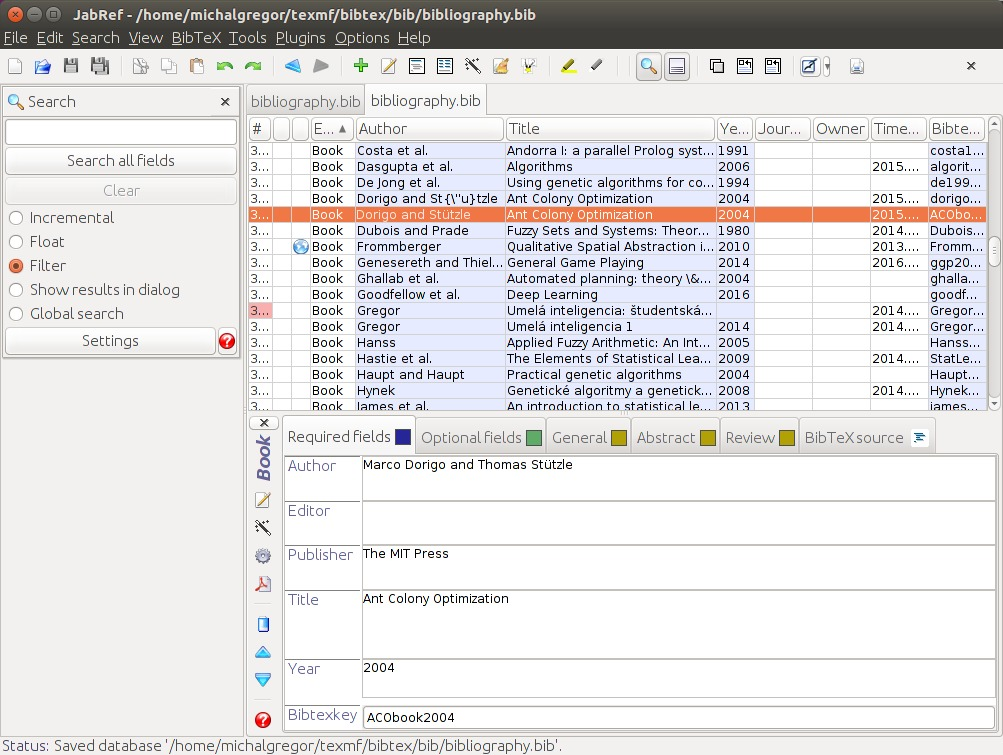
\includegraphics[width=14cm]{jabref}
\caption{Grafické rozhranie aplikácie JabRef.}
\label{fig:jabref}
\end{figure}

% !TeX spellcheck = sk_SK
\chapter{Typografia dokumentu}

V tejto časti špecifikujeme aj explicitne aspoň základné informácie o tom, ako je dokument štýlovaný. Okrem toho pripomenieme niektoré základné typografické zásady, ako je správne používanie spojovníkov, pomlčiek, medzier a pod.

\section{Štýl dokumentu}

Celý dokument využíva font v štýle Times New Roman -- konkrétne používame LaTeX balíčky \texttt{newtxtext} a \texttt{newtxmath}. Na realizáciu písma v štýle písacieho stroja (makro \texttt{{\textbackslash}texttt}) používame font \texttt{lmvtt}.

\subsection{Štýlovanie odsekov}

Všetky základné odseky používajú riadkovanie $\num{1.5}$. V LaTeX-u sa označuje ako dvojité riadkovanie (\angl{double spacing}). V niektorých špeciálnych kontextoch (ako poznámky pod čiarou a pod.) sa používa jednoduché riadkovanie.

Prvý riadok odsekov je odsadený zľava. Výnimku tvoria odseky nasledujúce priamo po nadpise -- tie nie sú odsadené.

\subsection{Štýlovanie strán}

Bežné strany v dokumente majú záhlavie a pätu. Záhlavie obsahuje nadpis aktuálnej kapitoly prvej úrovne. Päta obsahuje číslo strany.

Okraje strán sú nastavené nasledovne:
\begin{itemize}
\item horný okraj: $\num{11.25}$cm;
\item dolný okraj: $\num{1.5}$cm;
\item ľavý okraj: $\num{3}$cm;
\item pravý okraj: $\num{2.5}$cm.
\end{itemize}

Výška záhlavia strany je $1$cm, odstup medzi záhlavím strany a hlavným textom je $\num{0.75}$cm. Rozostup medzi spodnou hranicou hlavného textu a spodnou hranicou päty strany je $1$cm.

Osobitné formátovanie majú strany, na ktorých začína nová kapitola (prvej úrovne). Nová kapitola začína vždy na novej strane -- veľkým nadpisom. Preto tieto strany nemajú záhlavie, ktoré by predstavovalo zbytočnú duplicitu.

Odlišný formát majú aj strany v úvodnej (obsah, abstrakt, anotácia, zoznamy obrázkov a tabuliek, ...) a záverečnej časti práce (prílohová časť, ...) -- líšia sa predovšetkým číslovaním strán. V úvode sú strany číslované malými rímskymi číslami a v závere veľkými rímskymi číslami.

\section{Typografické zásady}
\label{sec:typograficke_zasady}

% Tu sú zámerne dva nadpisy tesne za sebou ako príklad.

\subsection{Spojovníky a pomlčky}
\label{sec:spojovniky_pomlcky}

Pripomíname, že spojovník \enquote{-} sa píše vždy vo vnútri slova a neoddeľuje sa medzerami, napr. čierno-biely (t.j. skladajúci sa z čiernej a z bielej časti).

Pomlčkami sa oddeľujú časti textu vo vete -- napr. môžu slúžiť na vkladanie poznámok, ako to ilustrujeme tu -- nepoužívajú sa vo vnútri slov. Pomlčka \enquote{--} je dlhšia než spojovník a z obidvoch strán sa oddeľuje medzerami. V LaTeX-u sa pomlčka píše pomocným zápisom \enquote{{-}{-}} -- každý výskyt tohto zástupného symbolu LaTeX nahradí regulárnou pomlčkou.

V iných jazykoch, napr. v angličtine, sa niekedy používa ešte dlhšia pomlčka \enquote{---}, ktorá má podobnú funkciu ako klasická pomlčka a typicky sa neoddeľuje medzerami. V slovenčine sa tento typ pomlčky typicky nepoužíva.

\subsection{Písanie medzier}

Na pripomenutie pre istotu uvádzame aj, že medzery sa nikdy nepíšu pred bodkou, čiarkou, bodkočiarkou, dvojbodkou a pod., ale len za nimi.

V slovenskej typografii sa píše medzera aj medzi číslami a označením jednotiek, resp. číslami a znakom percent \%, napr.:
\begin{itemize}
\item 22 cm;
\item 75 \%.
\end{itemize}
V angličtine sú pravidlá odlišné.

Medzery sa zvyknú písať aj pri udávaní rozsahov (napr. rokov alebo strán):
\begin{itemize}
\item s. 112 -- 125;
\item v rokoch 1928 -- 1932.
\end{itemize}
Tejto konvencie sa však nepridŕžajú všetci -- možno aj s ohľadom na to, že v českej typografii sa v týchto prípadoch medzery používať nezvyknú. Výnimku tvoria aj rozsahy strán v bibliografických záznamoch podľa normy ISO, ktoré sa píšu bez medzier.

\subsection{Viacero nadpisov za sebou}

Treba sa pridŕžať konvencie, že v texte by nemalo nasledovať viacero nadpisov bezprostredne za sebou -- ako to vidno vyššie, na nadpisoch \ref{sec:typograficke_zasady} a \ref{sec:spojovniky_pomlcky}. Za prvým nadpisom by namiesto toho mohlo nasledovať napríklad niekoľko viet stručne charakterizujúcich obsah danej podkapitoly.

%-------------------------------------------------------
%                     Bibliography
%-------------------------------------------------------

\printbibliography[heading=unchapter,title={Zoznam použitej literatúry}]

%-------------------------------------------------------
%					Čestné vyhlásenie
%-------------------------------------------------------

\makeDeclaration

%-------------------------------------------------------
%						Appendix
%-------------------------------------------------------

\makeAppendixPage
\appendix

\etoctocstyle{1}{Zoznam príloh}
\etocdepthtag.toc{mtappendix}
\etocsettagdepth{mtchapter}{none}
\etocsettagdepth{mtappendix}{subsection}
\tableofcontents

% !TeX spellcheck = sk_SK

\chapter{Zeleninový šalát}

Tvorba príloh je veľmi jednoduchá -- stačí ich pridať ako nové kapitoly v časti dokumentu označenej ako \texttt{{\textbackslash}appendix}. Prílohy sú automaticky číslované nie numericky, ale písmenami abecedy, čím sú dostatočne odlíšené od klasických kapitol. Ak práca obsahuje prílohy, šablóna automaticky vygeneruje titulný list oddeľujúci prílohovú časť práce od hlavnej časti práce.

\section{Textová vata}

\Blindtext


\end{document}
